\chapter{Estado del Arte}\label{chapter:state-of-the-art}

\section{Lengua de Señas}\label{section:state-of-the-art:sl}
La lengua de señas es el principal medio de comunicación para los sordos. Es un idioma que utiliza signos o señas en lugar de sonidos para comunicarse. Los signos se producen utilizando las manos, la cara y el cuerpo. Los mismos se usan en todo el mundo y existen más de 300 variantes.
Las lenguas de señas son todas diferentes, no son inteligibles entre sí, no son universales y tienen su propia gramática y sintaxis, las cuales difieren de las del lenguaje hablado.

\subsection{Escritura de señas Sutton}\label{subsection:state-of-the-art:sw}
Sutton SignWriting, comúnmente conocida como SignWriting, es un sistema de escritura de lenguas de señas desarrollado en 1974 por Valerie Sutton, una bailarina que, dos años antes, había desarrollado la escritura danzaria (DanceWriting). Es muy específica y visualmente icónica, tanto en las formas de los personajes, que son imágenes abstractas de las manos, la cara y el cuerpo, como en su disposición espacial en la página, que no sigue un orden secuencial como las letras que forman las palabras escritas. Algunas formas estandarizadas más nuevas se conocen como el Alfabeto Internacional de Escritura por Señas (ISWA, por sus siglas en inglés).

\subsubsection{Símbolos}\label{subsubsection:state-of-the-art:sl:symbols}

En SignWriting, se utiliza una combinación de símbolos icónicos para formas de manos, orientación, ubicaciones corporales, expresiones faciales, contactos y movimiento\brackcite{thiessen2011signwriting}\brackcite{suttonsignwriting} para representar palabras en lengua de señas.


La cantidad de símbolos es extensa y, a menudo, brinda múltiples formas de escribir un solo signo. Así como tomó muchos siglos para que la ortografía de los diversos idiomas se estandarizara, la ortografía en SignWriting aún no está estandarizada para ninguna lengua de señas.
 Sutton originalmente la diseñó para que se escribiera horizontalmente (de izquierda a derecha), como en su idioma nativo, y desde el punto de vista del observador, pero luego lo cambió a vertical (de arriba a abajo) y desde el punto de vista del firmante, para ajustarse a los deseos de los escritores sordos.\brackcite{signwriting}
 \begin{figure}[ht!]
    \centering
    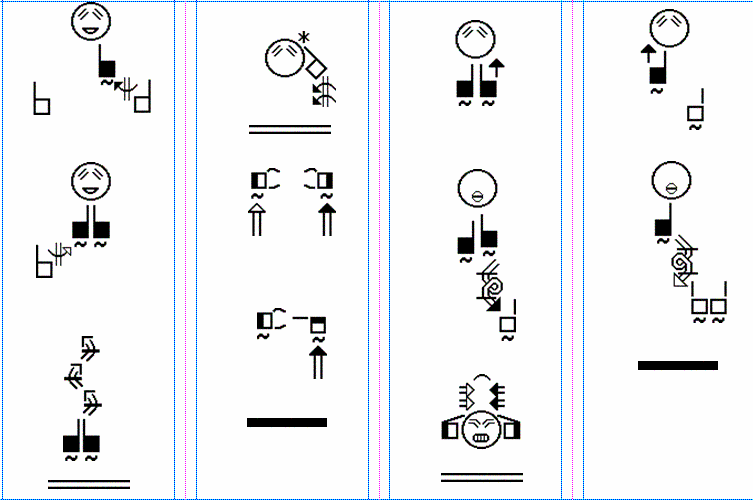
\includegraphics[width=0.6\textwidth]{Graphics/arreglo_glifos_sutton.png}
    \caption{Ejemplo de una secuencia de glifos del sistema de escritura de señas Sutton SignWriting. De manera vertical cada una de las cuatro secciones representa una seña}
    \label{fig:arreglo_glifos_sutton}
\end{figure}
 
 Dado que SignWriting representa la formación física real de los signos en lugar de su significado [Fig \ref{fig:arreglo_glifos_sutton}], no se requiere ningún análisis fonético o semántico de un idioma para escribirlo. Una persona que ha aprendido el sistema puede ``sentir'' un signo desconocido de la misma manera que una persona que habla inglés puede ``pronunciar'' una palabra desconocida escrita en el alfabeto latino, sin siquiera saber qué significa el signo.\brackcite{signwriting}

Las palabras pueden estar escritas desde el punto de vista del firmante o del espectador. Sin embargo, casi todas las publicaciones utilizan el punto de vista del firmante y asumen que la mano derecha es dominante. Existen varios símbolos de puntuación que corresponden a comas, puntos, signos de interrogación y exclamación y otros símbolos de puntuación de otras escrituras. Estos se escriben entre signos, y las líneas no se rompen entre un signo y su siguiente símbolo de puntuación.

La escritura de seña facilita enormemente la estandarización de las lenguas de señas, pero, a pesar de ello, no se encuentra popularizada globalmente y no se tiene constancia, al momento del autor realizar este trabajo, de que sea empleada en Cuba, por lo que otras alternativas como el reconocimiento de lenguas de señas pudieran ser de más utilidad.

\section{Reconocimiento de la Lengua de Señas}\label{section:state-of-the-art:slr}
El reconocimiento de la lengua de señas es ampliamente usado en diversos proyectos actualmente \brackcite{camgoz2020sign}. Se emplea en la identificación de gestos usando conjuntos de datos existentes
previamente. Las dos manos, la cabeza, los ojos, los
labios y el cuerpo  son, en esencia, lo utilizado en las lenguas de señas para realizar infinidad de gestos dedicados a funciones lingüísticas \brackcite{sandler2012dedicated}. Al ser los gestos una parte fundamental de este tipo de lenguas, se requiere de su reconocimiento específico. Los métodos de reconocimiento de gestos se pueden dividir en dos grandes grupos, en dependencia si utilizan un enfoque basado en hardware como Kinect u otros tipos de sensores, o un enfoque basado en software \brackcite{mitra2007gesture}. Dentro de este segundo enfoque destaca la detección de gestos por MediaPipe Holistic de Google, logrando muy buenos resultados en dichas tareas \brackcite{mediapipe_2020} [Fig \ref{fig:mediapipe}] .


\begin{figure}[ht!]
    \centering
    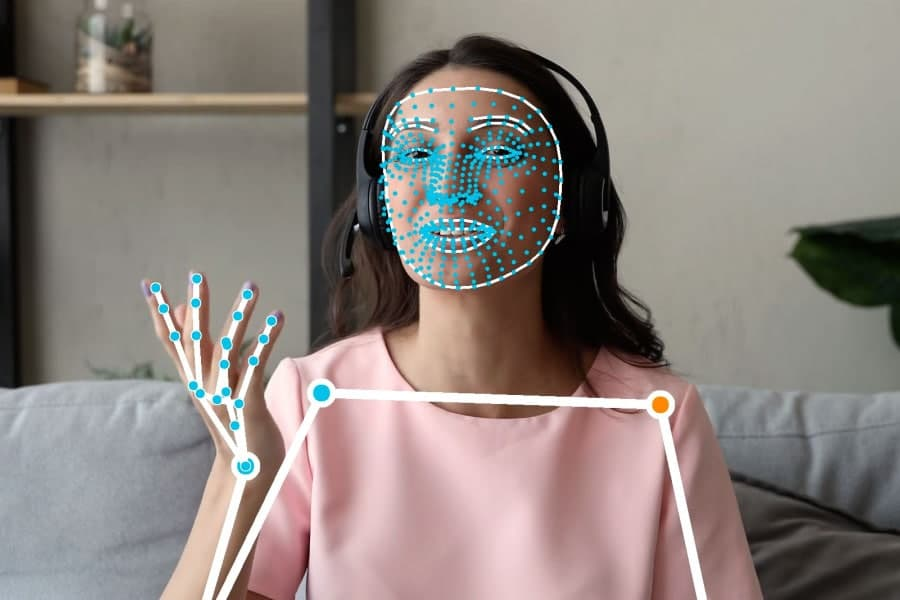
\includegraphics[width=0.6\textwidth]{Graphics/mediapipe.png}
    \caption{Software MediaPipe Holistic de Google, ejecutando un reconocimiento sobre una mujer.}
    \label{fig:mediapipe}
\end{figure}

Las diferentes vías de reconocimiento de señas aportan información valiosa para la comprensión kinética, estructural y lingüistica de cada lengua de señas. Esto ayuda en la comprensión en un sentido, del oyente hacia el hipoacúsico, ya que este último es entendido por el oyente pero no en el otro sentido. Es por ello que se hace necesario el uso de formas de reforzar el entendimiento de la persona sorda hacia el oyente.

\section{Tecnología de avatares}\label{section:state-of-the-art:avatars}

La traducción automática de lenguas de señas, aplicando la tecnología de generación de avatares, ha sido empleada en proyectos como ViSiCAST  y eSIGN [véase Fig \ref{fig:avatares-visicast}], apoyados por la Unión Europea \brackcite{visicast_at_uea_2021} \brackcite{esign_at_uea_2021}. Se utilizan para traducir de las lenguas habladas a las lenguas de señas, lo cual solamente concierne la parte del avatar en sí. Las animaciones para las señas individuales son generadas basándose en las señas no manuales de datos complementarios y en señas individuales. Los procesos para generar los avatares incluyen una serie de pasos bastante complejos.
 
\begin{figure}[ht!]
    \centering
    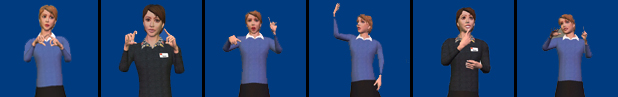
\includegraphics[width=0.6\textwidth]{Graphics/avatares_visicast.png}
    \caption{Muestra de los avatares de ViSiCAST, efectuando algunos movimientos}
    \label{fig:avatares-visicast}
\end{figure}

 
Los aspectos referentes a la velocidad, el ritmo y el tamaño deben ser tomados en
consideración utilizando reglas para controlarlos, ser configurados por un humano o
como resultado de un modelo de aprendizaje de máquina \brackcite{Nguyen2021AutomaticGO}. Otro de los usos que tienen estos métodos es lograr el anonimato en los videos y, cabe remarcar, que  son relativamente nuevos comparándolos con otros métodos de traducción automática de lenguas de señas \brackcite{kang2010effect} \brackcite{saragih2011real}.

Uno de los más grandes desafíos es que los avatares luzcan como humanos. En diversos estudios se comparan los gestos de los avatares con los gestos de los
humanos incluyendo algunos trabajos que han obtenido buenos resultados en Reino Unido en cuanto a generar dichos avatares con rasgos humanos utilizando modelos generativos \brackcite{stoll2018sign}. En Corea, usando el mismo corpus del trabajo anterior, se han logrado avances en un enfoque no auto-regresivo para lograr resultados incluso mejores \brackcite{hwang2021non}.

 Entre las tecnologías más utilizadas para la generación de avatares por animación se encuentran:
 \begin{itemize}
 \item  Unity
 \item Unreal 4
 \item Blender
 \item Maya3D 
 \item DirectX
 \end{itemize}  
 
 Se han desarrollado lenguajes de marcado para automatizar la generación de avatares de una forma dinámica y flexible \brackcite{latoschik2017effect} \brackcite{aneja2019high}. El estado del arte en la generación de avatares no está completamente automatizado, la mayoría de las partes del proceso de generación incluyen intervención humana para lograr buenos resultados. Gran parte de las investigaciones miden la calidad de las animaciones de avatares de forma perceptual y de estudios comprensivos con participantes sordos-mudos, incluyendo investigaciones metodológicas y recursos compartidos \brackcite{huenerfauth2006generating} \brackcite{kacorri2017regression}.
 
 En cuanto a la generación automática de avatares, han ocurrido recientes avances al poderse utilizar una interfaz de programación de aplicación de uno de los motores gráficos mencionados anteriormente. Se utilizan como medio para enlazar un archivo de captura de movimiento a una armadura predefinida en el motor gráfico, como por ejemplo una jerarquía de visión biótica (BVH, por sus siglas en inglés) a un diseño 3D de una persona \brackcite{Nguyen2021AutomaticGO}. Aún así, estas señas aisladas no son capaces de generar todo el vocabulario posible de la lengua de señas específica, por lo que convendría poseer una manera de crear cualquier secuencia de señas, dado un vocabulario establecido, mediante algún tipo de interpolación entre ellas.

\section{Modelos Generativos}
Durante la última década se ha visto un marcado incremento en lo que vienen siendo programas capaces de generar imágenes con un alto nivel de realismo, pero sin copiar nada de ninguna otra parte, siendo  ``auténticas'' de cierta forma. Esto es gracias a los denominados modelos generativos. Una nueva generación de modelos de redes neuronales capaces de aprender a hacer imágenes desde cero.\\

\subsection{Redes Generativas Adversariales}

Las Redes Generativas Adversariales (GANs) han logrado resultados impresionantes en varias tareas de síntesis de imágenes, y se están convirtiendo en un tema popular en la investigación de la visión por computadoras, debido al impresionante rendimiento que han alcanzado en diversas aplicaciones. Este modelo se ha impuesto desde que Goodfellow\brackcite{goodfellow2020generative} lo propuso en 2014.
Las GANs consisten en un generador G que se utiliza para generar muestras realistas a partir de ruido aleatorio e intenta engañar al discriminador D. El discriminador D se utiliza para identificar si la muestra es real o generada por G. El generador y el discriminador compiten entre sí hasta que el discriminador no puede distinguir entre las imágenes reales y las falsas [Fig \ref{fig:gan-design}].

\begin{figure}[ht!]
    \centering
    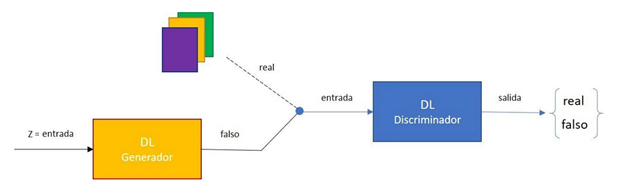
\includegraphics[width=0.6\textwidth]{Graphics/gan-design.png}
    \caption{Diseño de la arquitectura de redes adversariales generativas. En amarillo con una G se identifica al generador, mientras que el discriminante se identifica con el color azul y una D en el nombre. Arriba se puede apreciar la entrada de datos.}
    \label{fig:gan-design}
\end{figure}

\subsection{Redes Generativas Adversariales Condicionales}
Las GANs condicionales (CGAN) consisten en un Generador y Discriminador condicionados durante el entrenamiento mediante el uso de alguna información adicional [Fig \ref{fig:cgan-design}]. Esta información auxiliar podría ser, en teoría, cualquier cosa, como una etiqueta de clase, un conjunto de etiquetas o incluso una descripción escrita \brackcite{langr2019gans}. 
Durante el entrenamiento de CGAN, el Generador aprende a producir ejemplos realistas para cada etiqueta o descripción en el conjunto de datos de entrenamiento, y el Discriminador aprende a distinguir los pares ejemplo-etiqueta falsos de los pares ejemplo-etiqueta reales. \brackcite{langr2019gans}
Por lo tanto, para engañar al discriminador, no basta con que el generador de CGAN produzca datos de aspecto realista. Los ejemplos que genera también deben coincidir con sus etiquetas. Una vez que el Generador está completamente entrenado, nos permite especificar qué ejemplo queremos que sintetice el CGAN pasándole la etiqueta deseada.\brackcite{langr2019gans}

\begin{figure}[ht!]
    \centering
    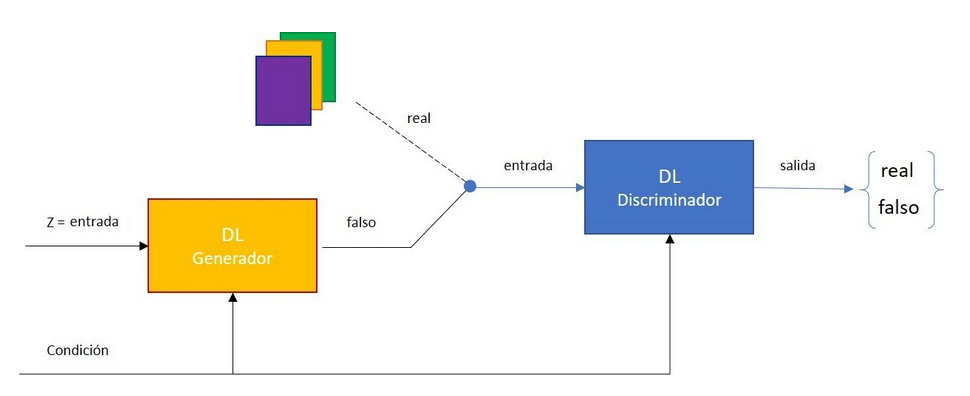
\includegraphics[width=0.6\textwidth]{Graphics/cgan-design.png}
    \caption{Diseño de la arquitectura de redes adversariales generativas condicionales. En amarillo con una G se identifica al generador, mientras que el discriminante se identifica con el color azul y una D en el nombre. Abajo de ellos se puede apreciar la entrada de datos}
    \label{fig:cgan-design}
\end{figure}

\subsection{Imágenes a partir de imágenes}
La traducción de imagen a imagen mediante redes generativas adversariales ha suscitado una gran atención en la investigación sobre el aprendizaje supervisado y no supervisado. Las GAN de ruido a imagen generan imágenes realistas a partir de muestras aleatorias de ruido, mientras que las GAN de imagen a imagen generan imágenes diversas a partir de imágenes. Se han propuesto muchas variantes de GAN, que han logrado buenos resultados en este tipo de tareas de traducción.
El objetivo de la traducción de imágenes es aprender el mapeo del dominio de la imagen de origen al de la imagen de destino, cambiando el estilo o algunas otras propiedades mientras mantiene el contenido de la imagen\brackcite{wang2020state}.
\subsubsection{Texto a imágenes}
En esta formulación, en lugar de utilizar ruido u otra imagen como entrada para el Generador, se utiliza una descripción textual de lo que se desea generar. Dicho texto es transformado primero en una incrustación (embedding) de texto, el cual se concatena con el vector de la imagen a generar y luego se da como entrada al Generador.  Esta formulación ayudará al Generador a crear imágenes alineadas con la descripción de entrada en lugar de generar imágenes aleatorias\brackcite{wang2020state}.

\subsection{Otras formas de generación de imágenes}
Existen otras formas de generación de imágenes como el \textit{image inpainting}, la cual es una técnica de restaurar y reconstruir partes de una imagen basadas en la información de fondo de la misma. La edición de imágenes, la cual manipula principalmente las imágenes a través del color e interacciones geométricas para completar tareas como la deformación y la mezcla de imágenes. Otra forma es la síntesis de imágenes humanas, la cual tiene como objetivo manipular la apariencia visual de las imágenes de los personajes, transfiriendo la pose de un personaje a la pose objetivo, que puede calcularse a partir de otros personajes.\brackcite{wang2020state}

Además, en el último año, se ha visto un fuerte incremento de la adopción masiva de los modelos de difusión para la generación de imágenes, siendo Stable Difussion \brackcite{rombach2021highresolution}, un modelo de difusión latente, el que encabeza el podio, quedando segundos, Dall-E y Midjourney (otros modelos de difusión) [Fig \ref{fig:stable-diffusion}]. Este éxito de Stable Diffusion se debe a que, tanto los pesos, como el código, se encuentran disponibles públicamente, siendo además eficiente y menos exigente que sus otros competidores, permitiendo ejecutarlo y obtener buenos resultados en máquinas modestas con al menos 8Gb de VRAM.

\begin{figure}[ht!]
    \centering
    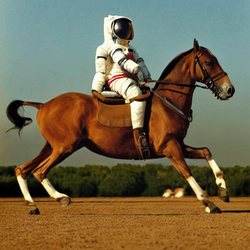
\includegraphics[width=0.6\textwidth]{Graphics/stable-diffusion.png}
    \caption{Imagen generada por Stable Diffusion}
    \label{fig:stable-diffusion}
\end{figure}

A pesar de poder ser capaces de hacer más realistas los vídeos de forma aislada (a través del uso de img2img) sigue siendo necesaria encontrar la forma de concatenar de manera fluida varias señas.

\section{Interpolación}\label{section:state-of-the-art:interpolation}
La interpolación es una forma de estimar datos nuevos en función de datos ya conocidos. Una técnica como esta puede ser aplicada para hacer predicciones en el campo de la economía y otras ramas. La dificultad con aplicarla en ese campo es la volatilidad del mismo que, sumado a los errores de precisión de la técnica, han llevado a los economistas a buscar otros métodos.\\

\subsection{Interpolación constante por partes}

El método de interpolación más simple es ubicar el valor de datos más cercano y asignar el mismo valor. En problemas simples, es poco probable que se use este método, ya que la interpolación lineal (ver a continuación) es más sencilla y devuelve mejores resultados con un menor número de puntos, pero en la interpolación multivariante de mayor dimensión, esta podría ser una opción favorable por su velocidad y simplicidad.


\subsection{Interpolación Lineal}
Una de las formas más simples es la interpolación lineal, la cual utiliza dos puntos ya conocidos $\left(x_{a}, y_{a} \right) $, $\left( x_{b}, y_{b}\right) $  y se usa la siguiente fórmula para estimar el punto $\left( x, y\right) $:
\begin{equation}
y = y_{a} + \left( y_{b} - y_{a}\right) \frac{x - x_{a}}{x_{b}-x_{a}}
\end{equation}
Esta ecuación anterior establece que la pendiente de la nueva recta entre $ \left(x_{a},y_{a}\right)$ y $\left(x ,y \right)$ es igual a la pendiente de la línea entre $\left(x_{a},y_{a}\right)$ y $\left(x_{b},y_{b}\right)$.\\

\subsection{Interpolación Cúbica}
Otra técnica de interpolación muy utilizada es la cúbica. Para utilizarla se necesita que la función $f\left( x \right) $ sea derivable y conocer los valores cuando $x=0$ y $x=1$, se utiliza un polinomio de grado tres y su derivada como se muestra a continuación:
\begin{align}
f\left( x \right) &= ax^3 + bx^2 + cx + d\\
f\prime\left( x \right) &= 3ax^2 + 2bx + c
\end{align}
Evaluando en los puntos $x=0$, $x=1$ y luego despejando se obtienen los siguientes valores:
\begin{align}
a &= 2f(0) - 2f(1) + f\prime(0) + f\prime(1)\\
b &= -3f(0) + 3f(1) - 2f\prime(0) - f\prime(1)\\
c &= f\prime(0)\\
d &= f(0)
\end{align}
Con eso se tiene todo lo necesario para la interpolación cúbica.\\
En caso de que no se conozca la derivada de la función,  se puede utilizar la derivada en puntos específicos. Si se tienen los puntos $\left(x_{0} ,p_{0} \right)$, $\left(x_{1} ,p_{1} \right)$,$\left(x_{2} ,p_{2} \right)$,$\left(x_{3} ,p_{3} \right)$:
\begin{align}
f(0) &= p_1\\
f(1) &= p_2\\
f\prime(0) &= \dfrac{p_2 - p_0}{2}\\
f\prime(1) &= \dfrac{p_3 - p_1}{2}
\end{align}
Combinando estos valores con la fórmula de la interpolación cúbica se obtiene:
\begin{align}
a &= -\tfrac{1}{2}p_0 + \tfrac{3}{2}p_1 - \tfrac{3}{2}p_2 + \tfrac{1}{2}p_3\\
b &= p_0 - \tfrac{5}{2}p_1 + 2p_2 - \tfrac{1}{2}p_3\\
c &= -\tfrac{1}{2}p_0 + \tfrac{1}{2}p_2\\
d &= p_1
\end{align}
Por lo que la fórmula de interpolación queda:
\begin{equation}
\begin{split}
f(p_0,p_1,p_2,p_3,x) &= (-\tfrac{1}{2}p_0 + \tfrac{3}{2}p_1 - \tfrac{3}{2}p_2 + \tfrac{1}{2}p_3)x^3 + \\ 
& (p_0 - \tfrac{5}{2}p_1 + 2p_2 - \tfrac{1}{2}p_3)x^2 + (-\tfrac{1}{2}p_0 + \tfrac{1}{2}p_2)x + p_1
\end{split}
\end{equation}
Esta forma de interpolar se conoce como Catmull-Rom spline.

\subsection{Otros métodos de interpolación}
Entre otros métodos que quedan sin comentar se encuentran:
\begin{itemize}

\item \textbf{La interpolación polinomial} la cual no es más que una generalización de la lineal y la cúbica.

\item \textbf{La interpolación por splines} que utiliza polinomios de bajo grado en cada uno de los intervalos y elige las piezas del polinomio de modo que encajen entre sí sin problemas. La función resultante es llamada spline.
 
\item \textbf{Interpolación mimética} la cual satisface las identidades del cálculo vectorial.

\end{itemize}

\subsection{Interpolación de movimiento}

La interpolación de movimiento (interpolación motriz) es una técnica de programación en la animación de personajes basada en datos que crea transiciones entre movimientos de ejemplo y extrapola nuevos movimientos.

Las acciones de ejemplo a menudo se crean a través de fotogramas clave o captura de movimiento. Sin embargo, la creación de fotogramas clave requiere mucha mano de obra y carece de variedades de movimiento, y ambos procesos dan como resultado movimientos que requieren mucho tiempo para modificarse. La interpolación motriz proporciona una alternativa mucho más rápida a la creación de nuevos movimientos a través de los mismos medios.\brackcite{Rose1998VerbsAA}


\section{Investigaciones y proyectos relacionados con la Lengua de Señas Cubana}\label{section:state-of-the-art:cubana}
En el área de las tecnologías de la información y las
comunicaciones sobre la Lengua de Señas Cubana  se pueden encontrar otros dos proyectos y/o trabajos.
 
 El desarrollo de una aplicación móvil [Fig. \ref{fig:app_cubana}] para dispositivos con sistema operativo Android, la cual esta enfocada en las familias con niños sordo-mudos, para brindarles el vocabulario necesario para interactuar con sus hijos \brackcite{android_app_lsc} y la tesis de grado referente al reconocimiento de la lengua de señas cubana usando métodos de traducción basados en inteligencia artificial y aprendizaje de máquina \brackcite{leynier-lsc-2021}.

\begin{figure}[ht!]
    \centering
    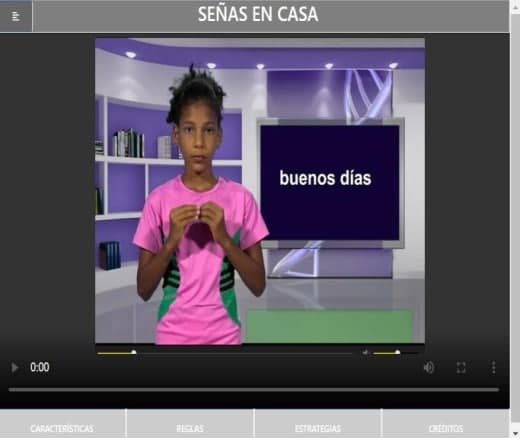
\includegraphics[width=0.6\textwidth]{Graphics/app_cubana.png}
    \caption{ Aplicación Android para la LSC \brackcite{android_app_lsc}}
    \label{fig:app_cubana}
\end{figure}

Se constata la existencia de una única investigación previa relacionada con la interpretación automática de la Lengua de Señas Cubana \brackcite{leynier-lsc-2021} pero ninguna en cuanto al tema que trata esta investigación.